\documentclass[9pt]{beamer}
% \documentclass[9pt,handout]{beamer}

\usepackage{ucs}
\usepackage[utf8x]{inputenc}
% \usepackage{beamerthemeplain}

\usepackage{amsmath}
\usepackage{amsfonts}
\usepackage{amssymb}
\usepackage[english]{babel}
\usepackage{fontenc}
% \usepackage{verbatim}
\usepackage{graphics}
 
\usepackage{textcomp}
\usepackage[absolute,overlay]{textpos}

\usepackage{wasysym}

\usepackage{slashed}
\usepackage{array}

\usetheme{CNRScolors}

\newcommand{\afac}[1]{\noindent \textcolor{red}{{\small \sc #1}}}

\usepackage{xspace}
%units
\usepackage[squaren,Gray,mediumqspace,thinspace,textstyle]{SIunits}

\usepackage[permil]{overpic}

\usepackage{textcomp}
\usepackage[absolute,overlay]{textpos}

\newcommand{\egamma}{E_{\gamma}}
\newcommand{\unitMass}{\giga\electronvolt/c^2}
\newcommand{\unitMom}{\giga\electronvolt/c}
\newcommand{\GeV}{\giga\electronvolt}
\newcommand{\TeV}{\tera\electronvolt}
\newcommand{\fb}{\femto\barn}
\newcommand{\pb}{\pico\barn}
\newcommand{\invmub}{\micro\reciprocal\barn}
\newcommand{\invpb}{\pico\reciprocal\barn}
\newcommand{\invfb}{\femto\reciprocal\barn}
\newcommand{\invnb}{\nano\reciprocal\barn}
\newcommand{\lumi}{\ensuremath{\mathcal{L}}}
\newcommand{\lumiunit}{\centi\meter\rpsquared\usk\reciprocal\second}
\newcommand{\pomeron}{\mathbb{P}}
\newcommand{\xp}{x_\pomeron}
\newcommand{\dkap}{\ensuremath{\Delta\kappa^{\gamma}}}
\newcommand{\kap}{\ensuremath{\kappa^{\gamma}}}
\newcommand{\lam}{\ensuremath{\lambda^{\gamma}}}
\newcommand{\aOw}{\ensuremath{a_0^W}}
\newcommand{\aOz}{\ensuremath{a_0^Z}}
\newcommand{\aCw}{\ensuremath{a_C^W}}
\newcommand{\aCz}{\ensuremath{a_C^Z}}
\newcommand{\aOwL}{\ensuremath{a_0^W/\Lambda^2}}
\newcommand{\aOzL}{\ensuremath{a_0^Z/\Lambda^2}}
\newcommand{\aCwL}{\ensuremath{a_C^W/\Lambda^2}}
\newcommand{\aCzL}{\ensuremath{a_C^Z/\Lambda^2}}
% \newcommand{\Lcutoff}{\ensuremath{\Lambda_{\text{cutoff}}}}
\newcommand{\Lcutoff}{\ensuremath{\Lambda}}
\newcommand{\wwgamma}{WW\gamma}
\newcommand{\missET}{\ensuremath{\not\!\!E_T}}
\newcommand{\etmiss}{\ensuremath{\not\!\!E_T}}
\newcommand{\WWgg}{\ensuremath{WW\gamma\gamma}}
\newcommand{\ggWW}{\ensuremath{WW\gamma\gamma}}
\newcommand{\dd}{\mathop{}\mathopen{}\text{d}}

\newcommand{\gpU}[1]{\ensuremath{\text{U}({#1})}}
\newcommand{\gpSU}[1]{\ensuremath{\text{SU}({#1})}}
\newcommand{\gpO}[1]{\ensuremath{\text{O}({#1})}}
\newcommand{\gpSO}[1]{\ensuremath{\text{SO}({#1})}}

\newcommand{\DO}{D\O{}\xspace}

\newcommand{\ith}{\textsuperscript{th}}
\newcommand{\st}{\textsuperscript{st}}
\newcommand{\nd}{\textsuperscript{nd}}
\newcommand{\rd}{\textsuperscript{rd}}

% \myfig[width=3cm]{label}{images/Chap1/myfig.pdf}{The capture of my figure.}
\newcommand{\myfig}[4][width=0.7\textwidth]{%
\begin{center}
 \begin{figure}
  \includegraphics[#1]{#3}
  
 \caption{\label{#2} #4}
 \end{figure}
\end{center}
}

\newcommand\FrameText[1]{%
  \begin{textblock*}{\paperwidth}(0pt,33pt)
    \raggedleft \small #1\hspace{.5em}
  \end{textblock*}}

\newcommand{\myincgr}[4]{
     \begin{overpic}[#1]{#2}
     \put(#3){#4}
     \end{overpic}}
\newcommand{\myincgrduo}[6]{
     \begin{overpic}[#1]{#2}
     \put(#3){#4}
     \put(#5){#6}
     \end{overpic}}
{\newcommand{\cmsSymbolFace}{\text}
\newcommand{\PT}{\ensuremath{p_{\text{T}}}\xspace}
\newcommand{\pt}{\ensuremath{p_{\text{T}}}\xspace}
\newcommand{\cm}{\ensuremath{\,\text{cm}}\xspace}
\newcommand{\PGm}{\ensuremath{\mu}\xspace} % muon
% \newcommand{\GeV}{\ensuremath{{\,\text{Ge\hspace{-.08em}V}}}\xspace}
\newcommand{\GeVc}{\ensuremath{{\,\text{Ge\hspace{-.08em}V\hspace{-0.16em}/\hspace{-0.08em}}c}}\xspace}
\newcommand{\GeVcc}{\ensuremath{{\,\text{Ge\hspace{-.08em}V\hspace{-0.16em}/\hspace{-0.08em}}c}^2}\xspace}
\newcommand{\abs}[1]{\ensuremath{\lvert #1 \rvert}}

% frequently used expressions
\newcommand{\ee}{\ensuremath{e^+e^-}\xspace}
\newcommand{\mumu}{\ensuremath{\mu^+\mu^-}\xspace}
\newcommand{\Mmumu}{\ensuremath{m_{\mu\mu}}\xspace}
\newcommand{\mmumu}{\ensuremath{m_{\mu\mu}}\xspace}
\newcommand{\eexp}[1]{\ensuremath{{\text e}^{#1}}\xspace}

% \newcommand{\qqbar}{\ensuremath{{\cmsSymbolFace{q}\overline{\cmsSymbolFace{q}}}}\xspace}
\newcommand{\QQbar}{\ensuremath{{\cmsSymbolFace{Q}\overline{\cmsSymbolFace{Q}}}}\xspace}
\newcommand{\Jpsi}{\ensuremath{\cmsSymbolFace{J}\hspace{-.08em}/\hspace{-.14em}\psi}\xspace}
\newcommand{\JPsi}{\ensuremath{\cmsSymbolFace{J}\hspace{-.08em}/\hspace{-.14em}\psi}\xspace}
\newcommand{\psiP}{\ensuremath{\psi\text{(2S)}}\xspace}
\newcommand{\B}{\ensuremath{\cmsSymbolFace{B}}\xspace}
\newcommand{\D}{\ensuremath{\cmsSymbolFace{D}}\xspace}

% \newcommand{\doubleRatio}{\ensuremath{\left.\left[N_{\psiP}/N_{\Jpsi}\right]_{\PbPb}\middle/\left[N_{\psiP}/N_{\Jpsi}\right]_{\pp}\right.\xspace}}
\newcommand{\doubleRatio}{\ensuremath{\left.(N_{\psiP}/N_{\Jpsi})_{\PbPb}/(N_{\psiP}/N_{\Jpsi})_{\pp}\right.\xspace}}

\newcommand{\PgU}{\ensuremath{\Upsilon}\xspace}
\newcommand{\PgUa}{\ensuremath{\Upsilon\text{(1S)}}\xspace}
\newcommand{\PgUb}{\ensuremath{\Upsilon\text{(2S)}}\xspace}
\newcommand{\PgUc}{\ensuremath{\Upsilon\text{(3S)}}\xspace}
\newcommand{\PgUbc}{\ensuremath{\Upsilon\text{(2S+3S)}}\xspace}
\newcommand{\PgUabc}{\ensuremath{\Upsilon\text{(1S,2S,3S)}}\xspace}
\newcommand{\PgUn}{\ensuremath{\Upsilon\text{(nS)}}\xspace}

\newcommand{\W}{\ensuremath{\cmsSymbolFace{W}}\xspace}
%\newcommand{\Z}{\ensuremath{\cmsSymbolFace{Z}}\xspace}
\newcommand{\ttbar}{\ensuremath{\cmsSymbolFace{t}\bar{\cmsSymbolFace{t}}}\xspace}

\newcommand{\dndy}{\ensuremath{dN/dy}\xspace}
\newcommand{\dnchdy}{\ensuremath{dN_{\text{ch}}/dy}\xspace}
\newcommand{\dndeta}{\ensuremath{dN/d\eta}\xspace}
\newcommand{\dnchdeta}{\ensuremath{dN_{\text{ch}}/d\eta}\xspace}
\newcommand{\dndpt}{\ensuremath{dN/d\pt}\xspace}
\newcommand{\dnchdpt}{\ensuremath{dN_{\text{ch}}/d\pt}\xspace}
\newcommand{\deta}{\ensuremath{\Delta\eta}\xspace}
\newcommand{\dphi}{\ensuremath{\Delta\phi}\xspace}
\newcommand{\phistar}{\ensuremath{\phi^*}\xspace}

\newcommand {\npart}  {\ensuremath{N_{\text{part}}}\xspace}
\newcommand {\ncoll}  {\ensuremath{N_{\text{coll}}}\xspace}

\newcommand{\AAA}{\ensuremath{\text{AA}}\xspace}
\newcommand{\raa}{\ensuremath{R_{\AAA}}\xspace}
\newcommand{\rpa}{\ensuremath{R_{\text{pA}}}\xspace}
\newcommand{\taa}{\ensuremath{T_{\AAA}}\xspace}
\newcommand{\rfb}{\ensuremath{R_\text{FB}}\xspace}

% references to equations, figures or tables
\newcommand{\eq}[1]{Eq.~\eqref{#1}\xspace}
\newcommand{\fig}[1]{Fig.~\ref{#1}\xspace}
\newcommand{\tab}[1]{Table~\ref{#1}\xspace}

% collision types
\newcommand{\pp}{{\ensuremath{\text{pp}}}\xspace}
\newcommand{\ppbar}{\ensuremath{\text{p}\overline{\text{p}}}\xspace}
\newcommand{\pPb}{\ensuremath{\text{p}\text{Pb}}\xspace}
\newcommand{\ppb}{\ensuremath{\text{p}\text{Pb}}\xspace}
\newcommand{\PbPb}{\ensuremath{\text{PbPb}}\xspace}
\newcommand{\pbpb}{\ensuremath{\text{PbPb}}\xspace}
\newcommand{\AuAu}{\ensuremath{\text{AuAu}}\xspace}

% center of mass energy
\newcommand{\sqrts}{\ensuremath{\sqrt{s}}\xspace}
\newcommand{\sqrtsnn}{\ensuremath{\sqrt{s_{_{\text{NN}}}}}\xspace}

%units
\newcommand{\mbinv} {\mbox{\ensuremath{\,\text{mb}^\text{$-$1}}}\xspace}
%\newcommand{\mubinv} {\mbox{\ensuremath{\,\mu\text{b}^\text{$-$1}}}\xspace}

% program name
\providecommand{\CASCADE} {{\textsc{cascade}}\xspace}
\providecommand{\HYDJET} {{\textsc{hydjet}}\xspace}


% ljpsi
\newcommand{\Lxy}{\ensuremath{L_{xy}}\xspace}
\newcommand{\Lxyz}{\ensuremath{L_{xyz}}\xspace}
% \newcommand{\ctau}{\ensuremath{c\tau^{2D}}\xspace}
% \newcommand{\ctauxyz}{\ensuremath{c\tau^{3D}}\xspace}
\newcommand{\ctau}{\ensuremath{\ell_{\Jpsi}^{2D}}\xspace}
\newcommand{\ctauxyz}{\ensuremath{\ell_{\Jpsi}^{3D}}\xspace}

% pPb 
\newcommand{\etalab}{\ensuremath{\eta_\text{lab}}\xspace}

\graphicspath{ {../figures/}{./} }

\setbeamertemplate{navigation symbols}{}

%%%%%%%%%%%%%%%%%%%%%%%%%%%%%%%%%%%%%%%%%%%%%%%%%%%%%%%%%
% \setbeameroption{show notes} % un-comment to see the notes
% \setbeamertemplate{note page}[plain]
%%%%%%%%%%%%%%%%%%%%%%%%%%%%%%%%%%%%%%%%%%%%%%%%%%%%%%%%%
\newif\ifmynote
% \mynotetrue
\mynotefalse
%%%%%%%%%%%%%%%%%%%%%%%%%%%%%%%%%%%%%%%%%%%%%%%%%%%%%%%%%
\newif\ifmyhide
% \myhidetrue
\myhidefalse
%%%%%%%%%%%%%%%%%%%%%%%%%%%%%%%%%%%%%%%%%%%%%%%%%%%%%%%%%

\newcommand\mynote[1]{%
\ifmynote \textbf{#1} \else \fi
}
\newcommand\myhide[1]{%
\ifmyhide \vspace{15pt} \begin{center} \myexample{(blackboard)}\end{center} \vspace{15pt} \else #1 \fi
}

 \newcolumntype{x}[1]{%
>{\centering\hspace{0pt}}p{#1}}%
\newcommand{\tn}{\tabularnewline}

\date[Stat2]{Sept. 27, 2018}
\title{Methods of statistical analysis and simulation}
\subtitle{2. Parameter estimation}
\author[E. Chapon]{Émilien Chapon}
% \institute[(CERN)]{CERN}
% \logo{\includegraphics[height=0.6cm]{../../CMS-Color-Label.pdf}\hspace{1.05\textwidth}\includegraphics[height=0.6cm]
% {../../LogoBadge.pdf} }

\begin{document}

{
\setbeamertemplate{footline}{}
\setbeamertemplate{headline}{}
% \logo{\includegraphics[height=1.2cm]{../../CMS-Color-Label.pdf}
% \hspace{0.94\textwidth}\includegraphics[height=1.2cm]{../../LogoBadge.pdf}}

\begin{frame}
 \maketitle
 
%  \setcounter{framenumber}{0}
\end{frame}
}


% CONTENU
% point estimation... cf cours ED, compléter avec le F. James

\begin{frame}
 \frametitle{Outline}
 
 \tableofcontents
\end{frame}

\section{Information}

\begin{frame}
 \frametitle{The likelihood function}
 
 
 We discuss a random variable $X$, with pdf $f(X|\theta)$, where $\theta$ is a real parameter (or a set of $k$ real parameters).
 The set of allowed values of $X$ is denoted $\Omega_\theta$.
 
\myhide{
 We consider $N$ independent observations of $X$: $X_1,\dots,X_N$. The joint pdf is, by independence,
 
 $$P(\vec{X}|\theta) = P(X1,\dots,X_N)|\theta) = \prod_{i=1}^N f(X_i|\theta)$$
 
 \begin{block}{Likelihood function}
  The likelihood function is a function of $\theta$, given the observed data $X^0$:
  
  $$\mathcal{L}(\theta) = P(X^0|\theta)$$
 \end{block}
 
}
  
\end{frame}

\begin{frame}
 \frametitle{Notes on the likelihood function}
 
 \begin{itemize}
  \item It is tempting to consider the area under $\mathcal{L}$, but $\mathcal{L}(\theta)$ is not a probability distribution function in $\theta$: \alert{the area under $\mathcal{L}$ is meaningless}.
  \item We will see that likelihood ratios are often used.
 \end{itemize}


\end{frame}

\begin{frame}
 \frametitle{Likelihood function: example}
 
 \begin{itemize}
  \item Poisson probability $P(n|\mu) = \mu^n \frac{e^{-\mu}}{n!}$
  \item Suppose $n=3$ is observed. We get the likelihood function:
  $$\mathcal{L}(\mu) = \mu^3 \frac{e^{-\mu}}{3!}$$
 \end{itemize}
 
 \begin{center}
  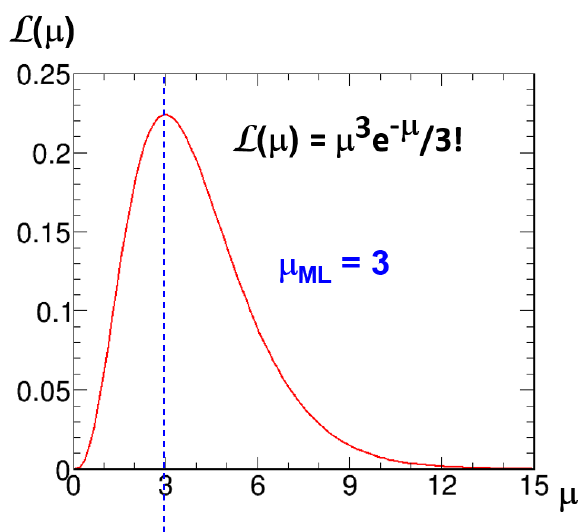
\includegraphics[width=0.6\textwidth]{likelihood_Poisson.png}
 \end{center}


\end{frame}


\begin{frame}
 \frametitle{Statistic}
 
 \begin{block}{Definition}
  Suppose a new random variable: $T = T(X_1,\dots,X_N)$. Any such function $T$ is called a \textbf{statistic}.
 \end{block}
 
 Example: sample mean $\bar{X}$.
 
 \vspace{10pt}
 
 NB: careful not to confuse this \textbf{statistic} with \textbf{statistics} (the field of mathematics we are discussing) or \textbf{statistics} (physicist's jargon as a substitute for
 ``data'' or ``amount of data''. Better avoid the latter usage when writing papers!

\end{frame}

\begin{frame}
 \frametitle{Information of R.A. Fisher}
 
 \begin{block}{Definition}
 \myhide{If $\Omega_\theta$ is independent of $\theta$, and if $\mathcal{L}(X|\theta)$ is regular enough to allow the operators $\partial^2/\partial\theta^2$ and $\int \dd X$ to comute, then
  \begin{eqnarray}
   I_X(\theta) & = & E \left[ \left( \frac{\partial \ln \mathcal{L}(X|\theta)}{\partial \theta} \right)^2 \right] \nonumber \\
   & = & \int_{\Omega_\theta} \left( \frac{\partial \ln \mathcal{L}(X|\theta)}{\partial \theta} \right)^2 \mathcal{L}(X|\theta) \dd X \nonumber \\
   & = & - E \left[ \frac{\partial^2 \ln \mathcal{L}(X|\theta)}{\partial \theta^2}  \right] \nonumber
  \end{eqnarray}
}
 \end{block}
 
 NB: this is an additive property (the information of $N$ observations is $N$ times the information of 1 observation).

\end{frame}


\begin{frame}
 \frametitle{Sufficient statistics}
 
 \begin{block}{Definition}
  A statistic is said to be \textbf{sufficient} if $f(\vec{X}|T)$ is independent of $\theta$.
 \end{block}
 
 Properties:
 
 \begin{itemize}
  \item<2-> If $T$ is a sufficient statistic for $\theta$, then any strictly monotonic function of $T$ is also a sufficient statistic for $\theta$.
  \item<3> $T(\vec{X})$ is a sufficient statistic for $\theta$ iff the likelihood factorises as
  $$\mathcal{L}(\vec{X}|\theta) = g(T,\theta) h(\vec{X}),$$
  where:
  \begin{enumerate}
   \item $h(\vec{X})$ does not depend on $\theta$
   \item $g(T,\theta) \propto A(T|\theta)$, the conditional pdf for $T$ given $\theta$.
  \end{enumerate}
 \end{itemize}


\end{frame}

\begin{frame}
 \frametitle{Darmois theorem}
 
 This theorem proves that only a very restricted class of probability density functions admits a number of sufficient statistics independent of the number of observations.
 
 \begin{itemize}
  \item<2-> Whatever $\Omega_\theta$, if there exists a number $N>1$ such that the set $X1,\dots,X_N$ admits a sufficient statistic for $\theta$, then the pdf is of the ``exponential form''
  $$f(X|\theta) = \exp [ \alpha(X)a(\theta) + \beta(X) + c(\theta)]$$
  \item<3> Inversely, $(X1,\dots,X_N)$ admits a sufficient statistic for all $N>1$ (but only if $\Omega_\theta$ does not depend on $\theta$), if $f(X|\theta)$ has the exponential form,
  and if the mapping $(X_1,\dots,X_N) \Rightarrow (R,X_2,\dots,X_N)$, with
  $$R = \sum_{i=1}^N \alpha(X_i),$$
  is one-to-one and continuously differentiable for all $X$. $R$ is sufficient for $\theta$, as well as any monotonic function of $R$.
 \end{itemize}

\end{frame}



\section{Parameter estimation on unbinned data}

\begin{frame}
 \frametitle{Outline}
 
 \tableofcontents[current]
\end{frame}


\begin{frame}
 \frametitle{Parameter estimation}
 
 Let $X$ be a random variable of pdf $f(x;\theta_0)$, with $\theta_0$ unknown. We draw $N$ independent trials of $X$, $\{x_1,\dots,x_N\}$.
 
 
 An \textbf{estimator} is a statistic $t_N(x_1,\dots,x_N)$ that can be used to estimate $\theta_0$. It can have the following properties:
 
 \mynote{Écrire au tableau le nom des différentes prioriétés, les afficher 1 par 1 au tableau}
 
 \begin{description}
  \item<2->[unbiased]: if $\langle t_N \rangle = \theta_0$ (otherwise the bias is $\langle t_N \rangle - \theta_0 = b_N$)
  \item<3->[convergent] or consistent: e.g. consistency in probability, $\forall \epsilon>0, \forall \eta>0, \exists N_0 / \forall N>N_0, P(|t_N - \theta_0|>\epsilon)<\eta$
  \begin{itemize}
   \item NB: The law of large numbers is equivalent to the statement that the sample mean is a consistent estimator of the parent mean.
  \end{itemize}
  \item<4->[efficient]: if the variance of the estimator $V(t_N) \xrightarrow[N\to\infty]{} \text{minimum variance bound}$ (this property can be only asymptotic)
  \item<5->[optimal]: if $t_N$ minimises the Mean Square Error (MSE): $\text{MSE}(t_N) = V(t_N) + b_N$
  \begin{itemize}
   \item NB: unbiasedness and efficiency imply optimality
  \end{itemize}
  \item<6>[robust]: if it does not depend on a hypothesis on the pdf
 \end{description}

\end{frame}

\begin{frame}
 \frametitle{Illustration}
 
 pdfs for $t_N$ in different cases
 
 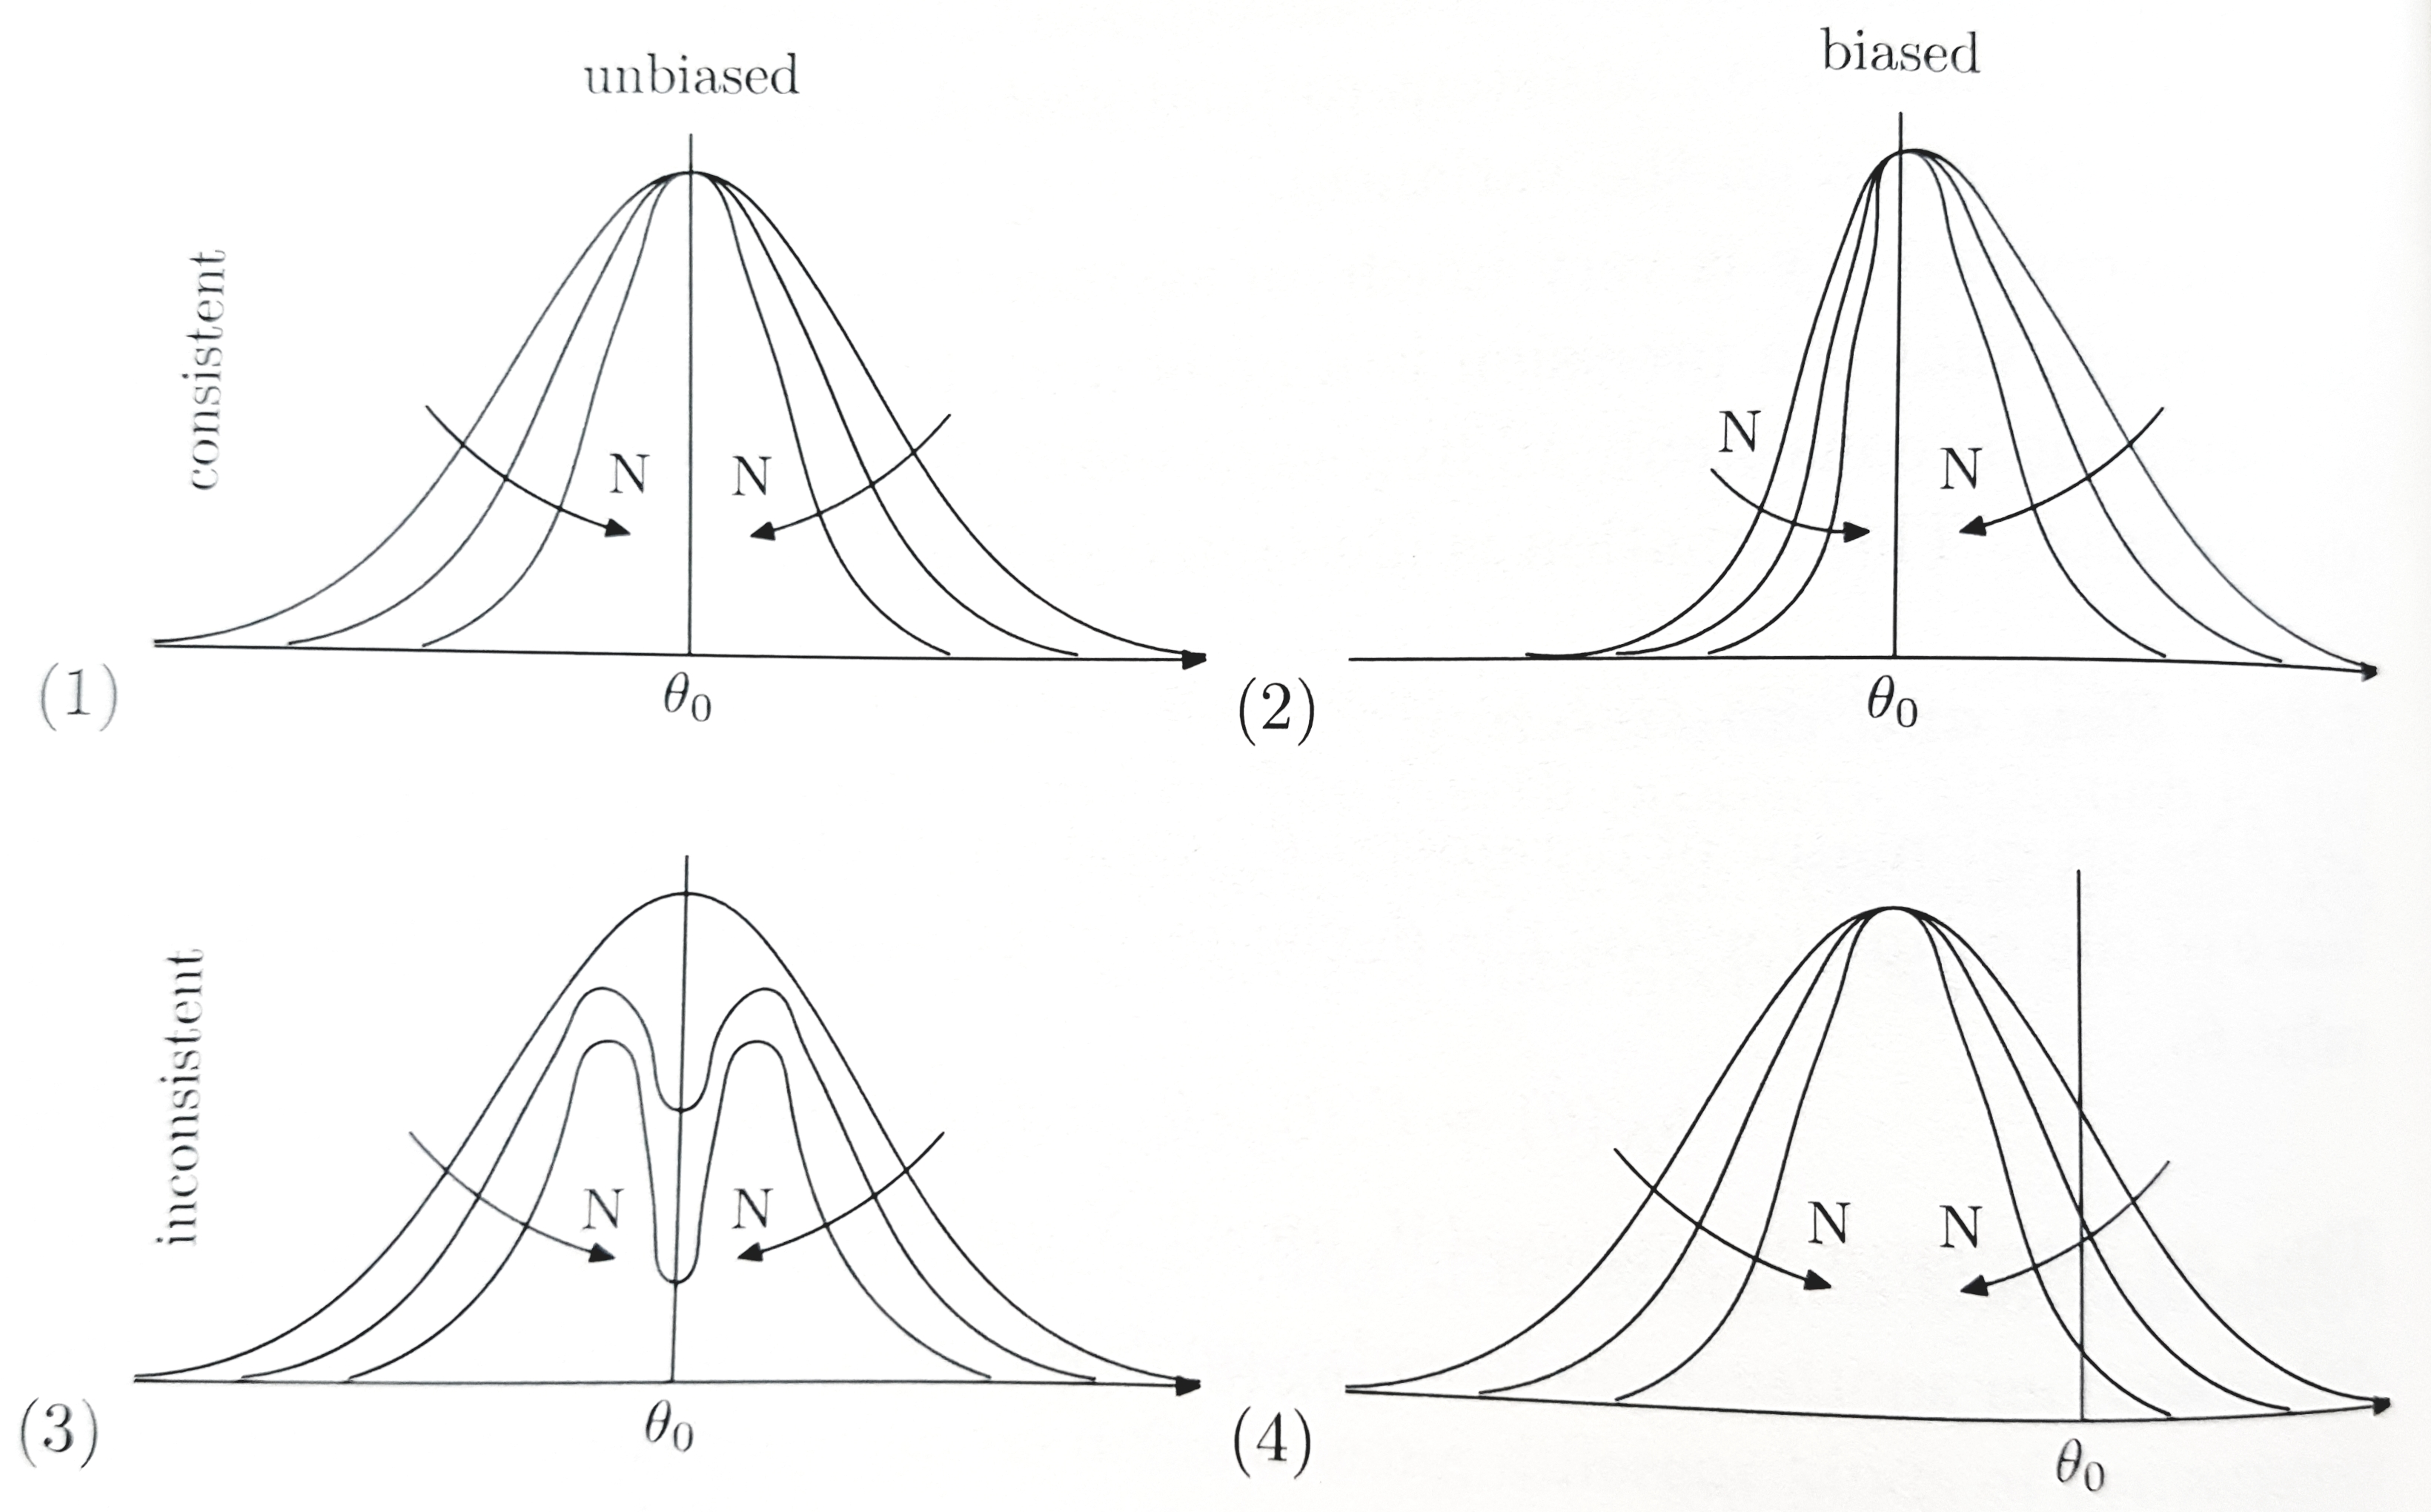
\includegraphics[width=\textwidth]{estimators.jpg}
\end{frame}


\begin{frame}
 \frametitle{Minimum variance: Cramér-Rao inequality}
 
 Let $\vec{X}$ be observations from a distribution with pdf $f(\vec{X}|\theta)$, the likelihood is $\mathcal{L}_{\vec{X}} = L(\vec{X}|\theta)$.
 
 \myhide{
 \begin{block}{Cramér-Rao inequality}
 If the range of $\vec{X}$ does not depend on $\theta$, and if $\mathcal{L}_{\vec{X}}$ is sufficiently regular that differentiation with respect fo $\theta$ and integration over 
 $\theta$ commute, then:
 
  $$V(\hat{\theta}) \geq \frac{[1+(\dd b / \dd \theta)]^2}{I_{\hat{\theta}}} 
  \geq \frac{[1+(\dd b / \dd \theta)]^2}{I_{\vec{X}}} 
  = \frac{\left( \frac{\dd \tau(\theta)}{\dd \theta} \right)^2}{E\left[ \left( \frac{\partial \ln \mathcal{L}_{\vec{X}}}{\partial \theta} \right)^2 \right]}$$
  
  where $I_{\vec{X}}$ is the Fisher information, $I_{\vec{X}}(\theta) = E\left[ \left( \frac{\partial \ln \mathcal{L}(\theta|\vec{X})}{\partial \theta} \right)^2 \right]$, and 
  $\tau(\theta) \equiv E(\hat{\theta}) = \theta + b(\theta)$
 \end{block}}

\end{frame}

\begin{frame}
 \frametitle{Efficiency and minimum variance}
 
 \begin{block}{First part of the inequality: minimum variance}
  $V(\hat{\theta}) = \frac{[1+(\dd b / \dd \theta)]^2}{I_{\hat{\theta}}} $ iff the sampling distribution of $\hat{\theta}$ is of the exponential form:
  
  $$\mathcal{L}_{\hat{\theta}} = \exp [a(\theta)\hat{\theta} + \beta(\hat{\theta}) + c(\theta)]$$
 \end{block}
 
 \uncover<2>{
 \begin{block}{Second part of the inequality: minimum bound variance (efficient estimator)}
  $V(\hat{\theta}) = \frac{[1+(\dd b / \dd \theta)]^2}{I_{\vec{X}}} $ iff $ I_{\hat{\theta}} = I_{\vec{X}} $, 
  
  ie iff $\hat{\theta}$ is a sufficient statistic for $\theta$, 
  
  ie  iff $f(\vec{X}|\theta)$ is of the exponential form (Darmois' theorem).
 \end{block}}


\end{frame}


\begin{frame}
 \frametitle{Usual methods of constructing consistent estimators}
 
 
 We will see:
 
 \begin{itemize}
  \item the moments method
  \item the maximum likelihood method
  \item the linear least squares method
 \end{itemize}
 
 \uncover<2>{NB: the last two are \textbf{implicitly defined estimators}, defined through an equation of the type $\xi(\hat{\theta})=0$}

 
\end{frame}

\subsection{Moments method}

\begin{frame}
 \frametitle{The moments method}
 
 We can use the law of large numbers:
 
 $$\frac{1}{N} \sum_{i=1}^N a(X_i) \xrightarrow[N\to\infty]{} E[a(X)] = \int a(X)f(X,\theta_0)\dd X$$
 
 Let $a(X)$ such that $E[a(X)] = \int a(X) f(X;\theta) \dd X = h(\theta)$ where $h$ is known. 
 
 If $h$ is invertible, we can find the true value of $\theta$: 
 $\theta_0 = h^{-1}(E[a]) = h^{-1}\left(\int a(X) f(X;\theta) \dd X\right)$
 
 \begin{block}{}
 The estimator is then:
 
 $$\hat{\theta} = h^{-1} \left( \frac{1}{N} \sum_{i=1}^N a(x_i) \right)$$
 \end{block}
 
 NB: $\hat{\theta}$ does not directly depend on $f$, only on the $x_i$: this is a \textbf{robust estimator}.
\end{frame}

\begin{frame}
 \frametitle{The moments method: application}
 
 \myhide{
 \begin{block}{1D case ($\theta \in \mathbb{R}$)}
  We take simply $a(X) = X$. Then $h(\theta_0) = \bar{X} = \mu$: it is the sample mean.
 \end{block}
 
 \begin{block}{ND case: $\vec{\theta} = (\theta_1,\dots,\theta_K)$}
  We take $a_j(X) = X^j$. Then $h_j(\vec{\theta}) = \mu_j(\vec{\theta})$: $j$-ith moment of $f(X;\vec{\theta})$
 \end{block}
}

\end{frame}



\subsection{Maximum likelihood method}

\begin{frame}
 \frametitle{The maximum likelihood method (ML)}
 
 \myhide{
 In general the logarithm of $\mathcal{L}$ is used: $\ln \mathcal{L}\left(\vec{X};\theta\right) = \sum_{i=1}^N \ln f(X_i;\theta)$
 
 \begin{block}{Maximum likelihood estimator}
  $$\left. \frac{\partial (\ln \mathcal{L} \left(\vec{X};\theta\right)}{\partial \theta}\right|_{\hat{\theta}_\text{ML}} = \left.\frac{\partial}{\partial \theta} \left(  \sum_{i=1}^N \ln f(X_i;\theta) \right)\right|_{\hat{\theta}_\text{ML}} = 0$$
  
  $\hat{\theta}_\text{ML}$ is the maximum likelihood estimator of $\theta$.
 \end{block}}

 \uncover<2>{Note: numerical methods are often designed to look for a minimum rather than a maximum. $-2 \ln \mathcal{L}$ is more commonly used.}
 
\end{frame}

\begin{frame}
 \frametitle{The maximum likelihood estimator (MLE)}
 
 This estimator is 
 \begin{itemize}
  \item<1-> \textbf{asymptotically efficient}
  \item<2-> \textbf{biased} (except when the likelihood is of the exponential form)
  \item<3-> \textbf{non optimal} (except when the likelihood is of the exponential form)
  \item<4-> \textbf{convergent}
  \item<5-> \textbf{invariant}: the ML estimate $\hat{\tau}$ of a function $\tau(\theta)$ is $\hat{\tau} = \tau(\hat{\theta})$
  \begin{itemize}
   \item However other properties of the MLE (e.g. the bias) are not invariant under change of parameter.
  \end{itemize}
  \item<6-> \textbf{not robust}: it requires to know the form of the PDF!
 \end{itemize}
 
 \uncover<7->{NB: invariance is an important and convenient property!}

\end{frame}

\begin{frame}
 \frametitle{Variance of the MLE}
 

 Because of asymptotic minimum variance bound:
 $$V(\hat{\theta}_{ML}) \xrightarrow[N\to\infty]{} \frac{1}{N} \left[ \left.-E\left(\frac{\partial^2\ln f(x;\theta)}{\partial \theta^2}\right)\right|_{\theta=\theta_0} \right]^{-1} \approx \frac{1}{D_2(\theta=\hat{\theta}_{ML})}$$
 
 \vspace{20pt}
 
 For finite samples, this can result in a misestimation of the variances. In the large sample limit (or in a linear model with Gaussian data), $\mathcal{L}$ is Gaussian and $\ln\mathcal{L}$ is (hyper)parabolic. Then contours with $s$ times the standarad deviations $\sigma_i$ can be found from the (hyper)surface defined by $\theta$ such that:
 
 $$\ln\mathcal{L}(\theta) = \ln\mathcal{L}(\hat{\theta}_\text{ML}) - s^2/2$$
 
 \uncover<2>{NB: $\ln(\mathcal{L}(\theta))$ can always be made parabolic through a change of variable, without changing the MLE, thanks to invariance.}
\end{frame}

\begin{frame}
 \frametitle{MLE: illustration for Gaussian data (unknown $\mu$, known $\sigma$)}
 
%  Plot $-\ln\mathcal{L}$, analytically, in 2 cases: a) Gaus, b) Poisson

 $$\mathcal{L}(\mu) = \frac{1}{\sqrt{2\pi}\sigma} e^{-\frac{(x-\mu)^2}{2\sigma^2}}$$
 
 $$-2\ln(\mathcal{L}(\mu)) = \frac{(x-\mu)^2}{\sigma^2} + \text{constant}$$
 
 \mynote{Jupyter here}
\end{frame}

\begin{frame}
 \frametitle{MLE: illustration for Poisson data}
 
 \mynote{Exercise}
 
 $$\mathcal{L}(\mu) = \mu^N \frac{e^{-\mu}}{N!}$$
 
 $$-2\ln(\mathcal{L}(\mu)) = -2 \times \left(N \times \ln \mu - \mu \right) + \text{constant} $$
 
 \begin{exampleblock}{}
  \begin{itemize}
   \item What is the MLE?
   \item What is the variance of the MLE? How does it compare to the minimum variance bound?
%    \item Compare to the value of $\mu$ such that $$-2 \times \ln\mathcal{L}(\theta) = -2\times\ln\mathcal{L}(\hat{\theta}_\text{ML}) +1$$
  \end{itemize}

 \end{exampleblock}
 
 \mynote{Jupyter here, + solving in the blackboard. $I_N(\mu) = E(-\frac{\partial^2}{\partial\mu^2} \ln \mathcal{L}(\mu|N)) = E(N/\mu^2) = 1/\mu$}

\end{frame}

\begin{frame}
 \frametitle{MLE: likelihood scans}
 
 From the CMS Higgs boson mass measurement (\href{http://cms-results.web.cern.ch/cms-results/public-results/publications/HIG-14-009/index.html}{EPJC 75 (2015) 212}):
 
 \begin{center}
  \includegraphics[width=0.7\textwidth]{CMS-HIG-14-009_Figure_002-a}
 \end{center}

\end{frame}



\begin{frame}
 \frametitle{(Academic) example of a poor MLE}
 
 \mynote{Exercise}
 
 \begin{exampleblock}{}
  A random variable $X$ is uniformly distributed on the interval $[0,\theta]$. $N$ indpendent trials $\{x_i\}$ are drawn. What is the MLE? Can you think of a better estimate?
 \end{exampleblock}
 
 \uncover<2->{
 \begin{itemize}
  \item The likelihood function is $\mathcal{L} = \prod_{i=1}^N \theta^{-1} = \theta^{-N}$ and the MLE is $\hat{\theta} = \max\{X_i\}$.
  \item<3-> The MLE is biased (always too small by definition)... intuitively $\hat{\theta}_{CS} = \max\{X_i\} + \max\{X_i\}/N$ is a better estimate.
 \end{itemize}
 }
\end{frame}

\begin{frame}
 \frametitle{(Academic) example of a poor MLE}
 
 \begin{center}
  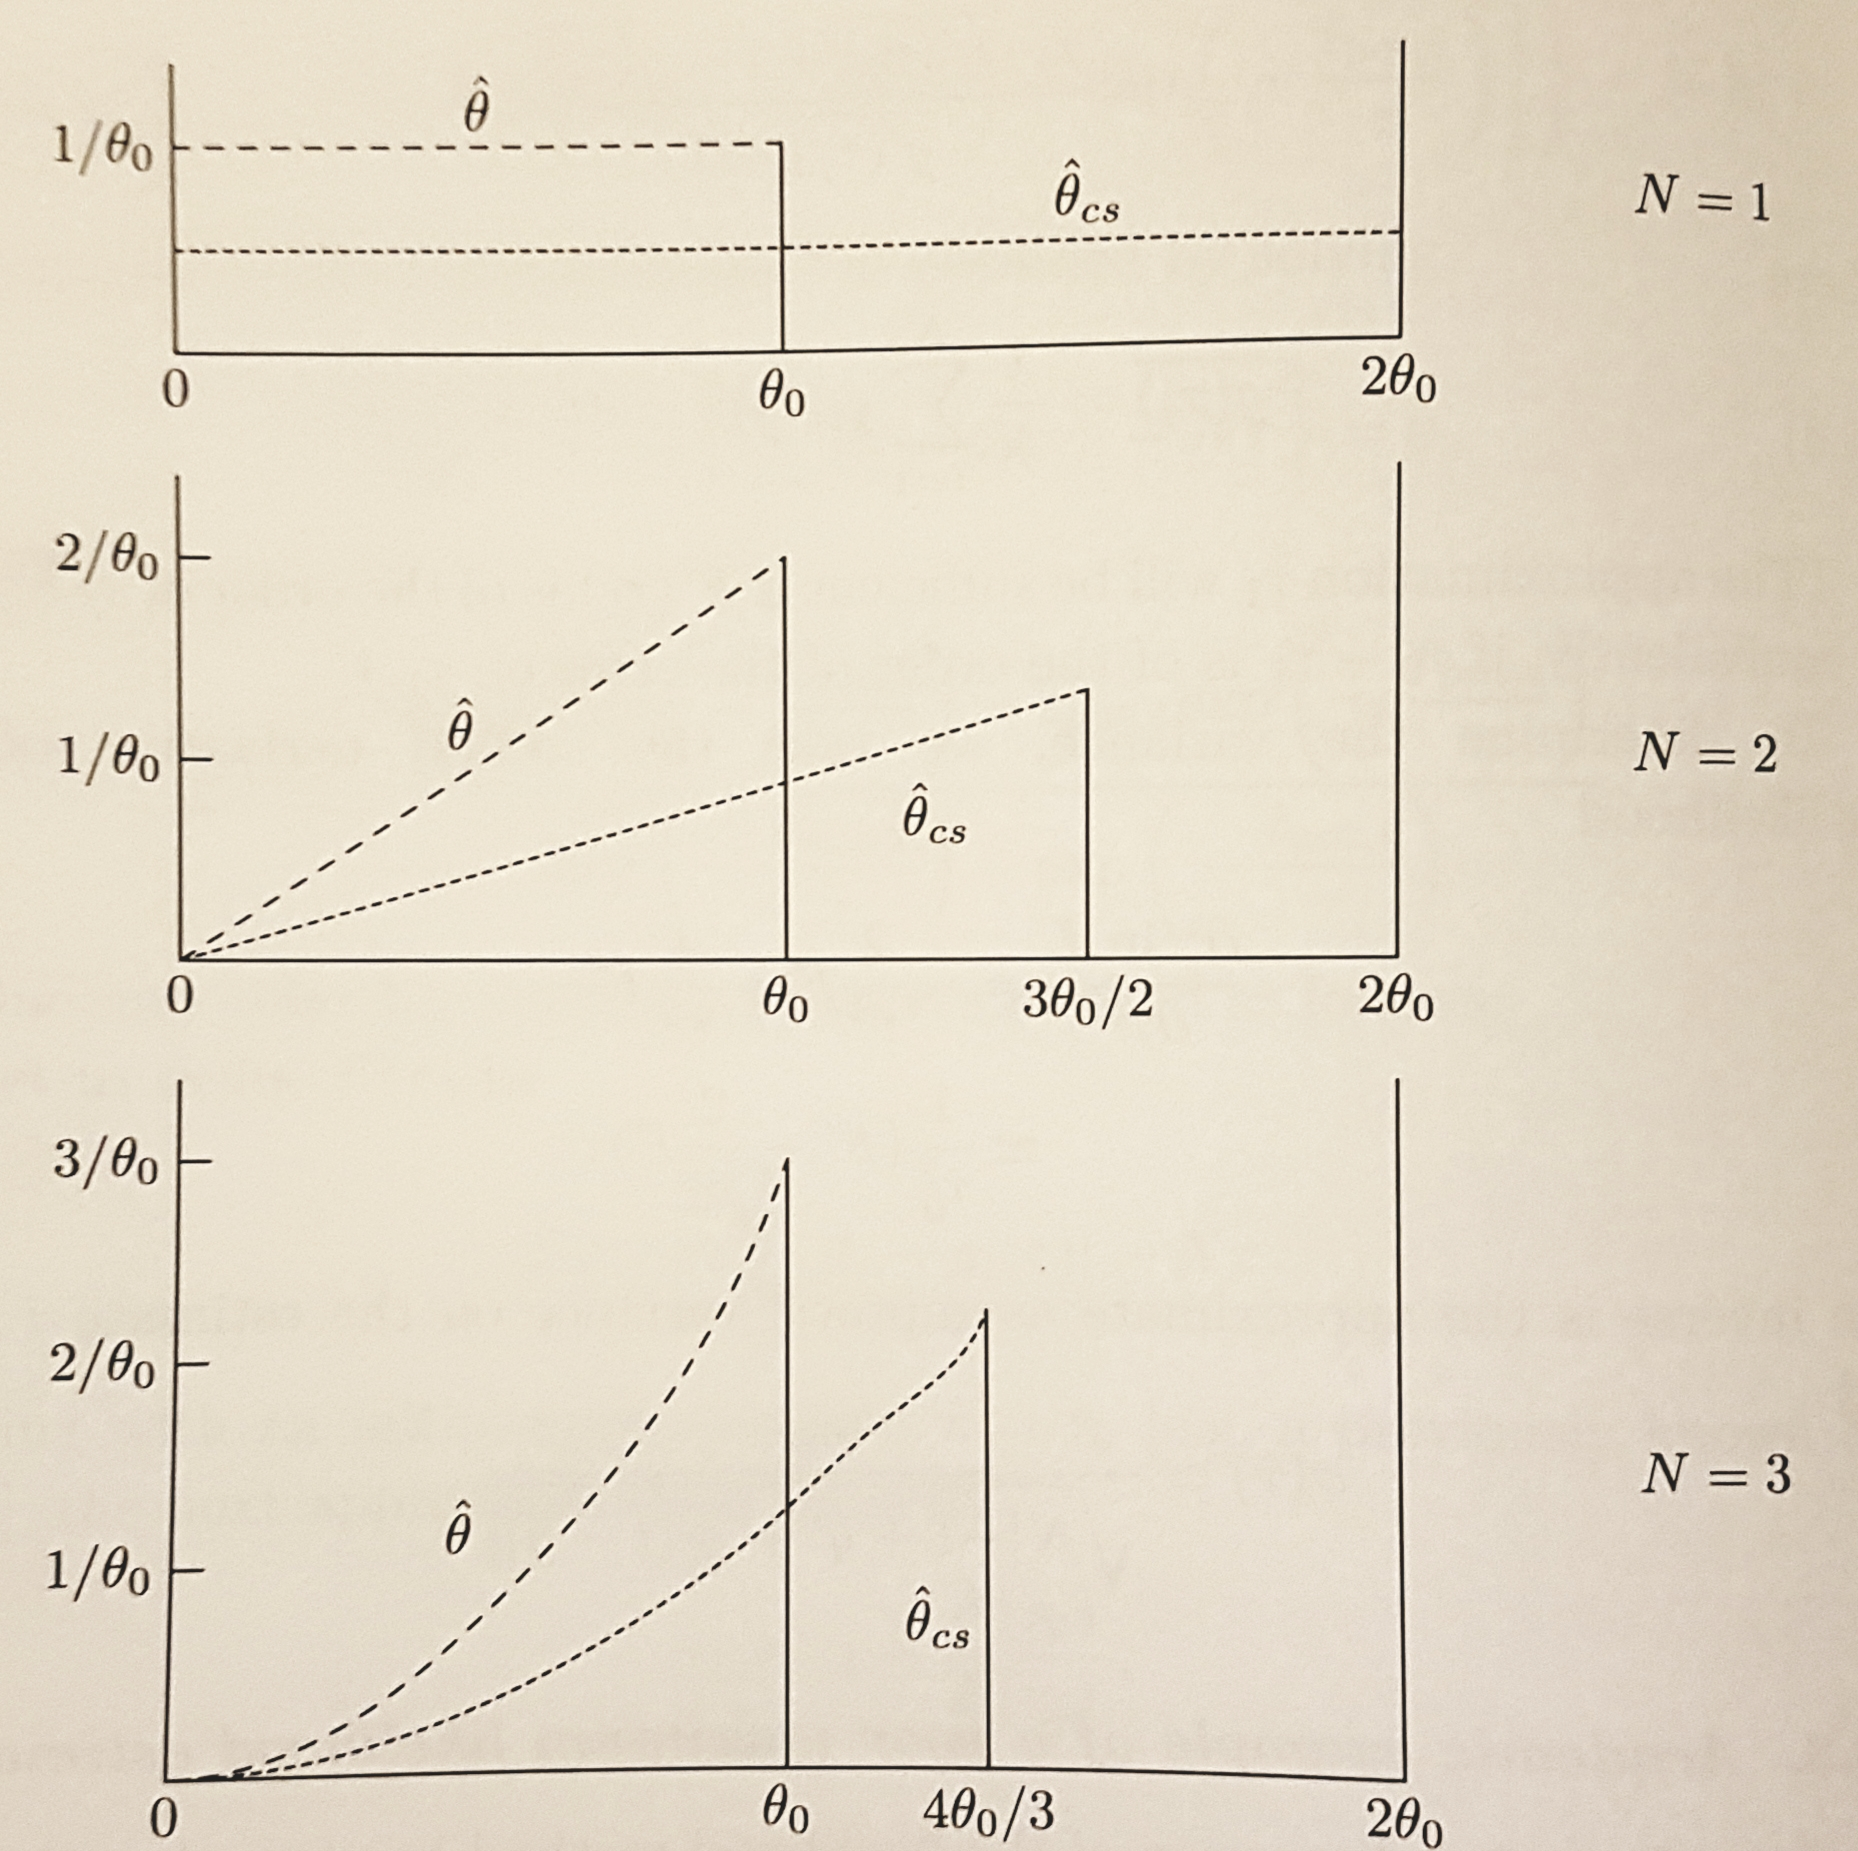
\includegraphics[width=0.7\textwidth]{academic_MLE.jpg}
 \end{center}

\end{frame}



\subsection{Least squares method}

\begin{frame}
 \frametitle{Outline}
 
 \tableofcontents[current]
\end{frame}

\begin{frame}
 \frametitle{Least squares method (aka $\chi^2$ estimator)}
 
 We consider $N$ observations $\vec{x}$
 
 $E(x_i;\vec{\theta})$ is a  and $V_{ij}$ ($i,j = 1\dots N$) are \textbf{known functions} of $\vec{\theta}$
 
 \myhide{
 \begin{block}{Least squares estimator}
 The estimator is the value $\vec{\theta}$ such that $Q$ is minimum:
 
  $$Q = \left[ \vec{X} - E(\vec{X};\vec{\theta}\right]^\intercal V^{-1} (\vec{\theta}) \left[ \vec{X} - E(\vec{X};\vec{\theta}) \right]$$
  
  $$Q = \sum_{i=1}^N \sum_{j=1}^N \left[ X_i - E(X_i;\vec{\theta})\right] V^{-1}_{ij} \left[ X_j - E(X_j;\vec{\theta})\right]$$
 \end{block}
 }
 
 \uncover<2>{
 This estimator is:
 
 \begin{itemize}
  \item \textbf{consistent}
  \item (generally) \textbf{biased}
  \item \textbf{non-optimal}
 \end{itemize}
}

\end{frame}

\begin{frame}
 \frametitle{Gaussian case}
 
 In the Gaussian case, the least squares and maximum likelihood methods coincide. 
 
 Assuming $N$ independent measurements $y_i$ at known points $x_i$, Gaussian distributed with mean
 $\mu(x_i;\theta)$ and known variance $\sigma_i^2$:
 
 $$\chi^2(\theta) = -2\ln\mathcal{L}(\theta) + \text{constant} = \sum_{i=1}^N \frac{\left(X_i - \mu(\theta)\right)^2}{\sigma_i^2}$$
\end{frame}


\begin{frame}
 \frametitle{$\chi^2$ estimator: uncorrelated case}
 
 \myhide{
 Uncorrelated case: $V_{ij} = 0 $ for $i \neq j$
 
 $$Q = \sum_{i=1}^N \frac{\left(x_i - E(x_i; \vec{\theta})\right)^2}{\sigma_i^2(\vec{\theta})}$$}
\end{frame}

\begin{frame}
 \frametitle{Variance of the $\chi^2$ estimator}
 
 \myhide{
 If $\theta \in \mathbb{R}$:
 
 $$V(\hat{\theta}_{LS}) \xrightarrow[N\to\infty]{} 2\left(\left.\frac{\partial^2 Q}{\partial\theta^2}\right|_{\theta=\theta_0}\right)^{-1} \approx \frac{2}{D_2(\theta=\hat{\theta}_{LS})}$$
 }
\end{frame}


\begin{frame}
 \frametitle{Specific cases of the $\chi^2$ estimator}
 
 \begin{block}{Linear case}
  If \structure{$\sigma_i$ are independent of $\theta$, and $E(x_k;\theta)$ linear function of $\theta$}: $Q$ is \textbf{optimal} and \textbf{convergent}.
 \end{block}
 
 \uncover<2->{
 \begin{block}{Gaussian case}
 
 \begin{itemize}
  \item If \structure{the $x_i$ follow a normal law $G(X_i;\mu_i,\sigma_i)$}: $Q$ follows a $\chi^2$ law, $\chi^2(Q;N)$:
  
  $$\chi^2(\vec{\theta}) = \sum_{i=1}^N \frac{\left( X_i - \mu_i (\vec{\theta})\right)^2}{\sigma_i^2 (\vec{\theta})}$$
  \item<3>If in addition \structure{the model is linear ($\sigma_i$ independent of $\theta$)}: $\chi^2_\text{min} = \chi^2 (\chi^2_\text{min};N-r)$ (with $r$ the dimension of $\vec{\theta}$), and $\vec{\theta}_{LS}$ follows a normal law of dimension $r$ with $\langle \hat{\theta}_{LS}\rangle = \vec{\theta}_0$, $V = 2 D_2^{-1}$
  
  $N-r$ is \textbf{the number of degrees of freedom}.
 \end{itemize}
  
 \end{block}}


\end{frame}

\section{Parameter estimation with histograms}

\begin{frame}
 \frametitle{Outline}
 
 \tableofcontents[current]
\end{frame}

\begin{frame}
 \frametitle{Histograms}
 
 Let's assume an histogram with $N$ uncorrelated bins (the total number of events is not fixed): $d_i$ events in bin $i$, with $i = 1 \dots N$. The $d_i$ follow Poisson laws: $E(d_i;\theta) = f_i(\theta)$,
 $\sigma^2(d_i;\theta) = f_i(\theta)$.
 
 \vspace{10pt}
 
 \begin{center}
  \includegraphics[width=0.8\textwidth]{histo}
 \end{center}

\end{frame}


\begin{frame}
 \frametitle{Usual methods for fitting histograms}
 
 \myhide{
 \begin{block}{Minimum $\chi^2$ method (expected uncertainties)} 
 \vspace{-7pt}
  $$Q_P = \sum_{i=1}^N = \frac{\left(d_i - f_i\right)^2}{f_i^2}$$
  \vspace{-7pt}
 \end{block}
 
 \begin{block}{Modified minimum $\chi^2$ method (observed uncertainties)} 
 \vspace{-7pt}
  $$Q_N = \sum_{i=1}^N = \frac{\left(d_i - f_i\right)^2}{d_i^2}$$
  \vspace{-7pt}
 \end{block}
 
 \begin{block}{Binned likelihood (multinomial data)}
 \vspace{-7pt}
  $$\ln \lambda = - \sum_{i=1}^N d_i \ln (d_i/f_i) = \sum_{i=1}^N d_i \ln (f_i) + \text{constant}$$
  \vspace{-7pt}
 \end{block}

\begin{block}{Binned likelihood (Poisson data)}
\vspace{-7pt}
  $$\ln \lambda = - \sum_{i=1}^N f_i - d_i + d_i \ln (d_i/f_i) = - \sum_{i=1}^N f_i - d_i \ln (f_i) + \text{constant}$$
  \vspace{-7pt}
 \end{block}}

\end{frame}

\begin{frame}
 \frametitle{}
 
 All methods are asymptotically equivalent. The binned likelihood method converges faster (and the modified $\chi^2$ is the slowest), and is less sensitive to empty bins. 
\end{frame}

\section{Some basic estimators}


\begin{frame}
 \frametitle{Outline}
 
 \tableofcontents[current]
\end{frame}

\begin{frame}
 \frametitle{Sample mean}
 
 \mynote{Écrire d'abord au tableau}
 
 \uncover<2>{
 $$\bar{X} = \sum_{i=1}^N \frac{x_i}{N} = \bar{\mu}$$
 
 This estimator is \textbf{unbiased}, thanks to the central limit theorem.
 
 Its variance is:
 
 $$V(\hat{\mu}) = \frac{\sigma^2}{N},\qquad\text{i.e.}\quad \sigma(\hat{\mu}) = \frac{\mu}{\sqrt{N}}$$
 
 The sample mean is an \textbf{efficient estimator} of the mean of a Gaussian, but not in the general case.
 }
\end{frame}

\begin{frame}
 \frametitle{Variance estimator: known mean}
 
 \mynote{Écrire d'abord au tableau}
 
 \uncover<2>{
 $$\hat{V}_\mu = \frac{1}{N} \sum_{i=1}^N (x_i-\mu)^2$$
 
 This estimator is \textbf{consistent and unbiased}: $\langle \hat{V}_\mu \rangle = \frac{N\langle (x-\mu)^2 \rangle}{N} = V$
 }
\end{frame}

\begin{frame}
 \frametitle{Variance estimator: unknown mean}
 
 \myhide{
 Using $\hat{\mu} = \bar{X}$
 
 $$\hat{V}_b = \frac{1}{N} \sum_{i=1}^N (x_i-\bar{X})^2 = \frac{1}{N} \sum_{i=1}^N (x_i^2 - \bar{X}^2)$$
 
 \begin{eqnarray}
  \langle \hat{V}_b \rangle & = & \frac{N \langle X^2 - \bar{X}^2 \rangle}{N} = \langle X^2 \rangle - \langle \bar{X} \rangle^2 \nonumber \\
  & = & \langle X^2 \rangle - \langle X \rangle^2 - \left( \langle \bar{X}^2 \rangle - \langle \bar{X} \rangle ^2 \right) \nonumber \\
  & = & V(X) - V(\bar{X}) \nonumber \\
  & = & V(X) - \frac{V(X)}{N} \nonumber \\
  & = & \left( 1 - \frac{1}{N} \right) V(X)\quad \neq V(X) \nonumber
 \end{eqnarray}
 
 This estimator is biased! $\rightarrow$ \textbf{Bessel correction}
 }

\end{frame}

\begin{frame}
 \frametitle{Variance estimator: unknown mean}
 
 \mynote{Écrire d'abord au tableau}

 \begin{block}{}
  $$\hat{V} = \frac{1}{N-1} \sum_{i=1}^N (x_i - \bar{X})^2$$
 \end{block}
 
 $$V(\hat{V}) = \frac{2V}{N}$$

\end{frame}

\section{Point estimation in practice}

\begin{frame}
 \frametitle{Outline}
 
 \tableofcontents[current]
\end{frame}

\begin{frame}
 \frametitle{Choice of estimator}
 \structure{How to choose an estimator?} It should have the following properties:
 
 \begin{itemize}
  \item<2-> Consistency and unbiasedness
  \item<3-> Minimum loss of information
  \item<4-> Minimum variance (efficient estimator)
  \item<5-> Robustness
  \item<6-> Simplicity (e.g. if possible normally distributed, etc.)
  \item<7-> Minimum computer time
  \item<8-> Minimum loss of physicist's time
 \end{itemize}

\end{frame}

\begin{frame}
 \frametitle{Monte-Carlo (``toy'') studies}
 
 \begin{block}{}
  Monte-Carlo studies: directly related to the frequentist paradigm (simulate experiment many times to estimate pdf)
 \end{block}

 
It is possible to write simple, short, fast Monte Carlo programs
that generate data for fitting.   Can then look at fit values, 
uncertainties, and pulls.  These are often called “toy” Monte 
Carlos to differentiate them from complicated event and detector
simulation programs.

\begin{itemize}
 \item Tests likelihood function.
 \item Tests for bias.
 \item Tests that uncertainty from fit is correct.
\end{itemize}

\uncover<2>{
This does NOT test the correctness of the model of the data.  For 
example, if you think that some data is 
Gaussian 
distributed, but 
it is really 
Lorentzian, then the simple Monte Carlo test will not reveal this.}
\end{frame}

% \begin{frame}
%  \frametitle{Simple Monte Carlo}
%  
%  \begin{exampleblock}{Exercise}
%   \begin{itemize}
%    \item Generate exponential ($\tau_0=0.5$ and $N=1000$)
%    \item Find MLE
%    \item Repeat many times (e.g. 1000 times)
%    \item Plot $\hat{\tau}$%, $\sigma(\hat{\tau})$, pulls ($= (\hat{\tau}-\tau_0)/\sigma(\hat{\tau})$) in histograms
%    \item Repeat for other estimators, especially binned
%   \end{itemize}
%  \end{exampleblock}
% 
% \end{frame}



% \subsection{More realistic cases}

% cf Fred James + PDG stat review

\begin{frame}
 \frametitle{Extended likelihood}
 
 In many cases the number of events $n$ is not fixed: this dependence should be included in the likelihood: this is called the extended likelihood.
 
 \myhide{$$\mathcal{L}(\vec{\theta}) = \structure{\frac{\mu^n}{n!}e^{-\mu}} \prod_{i=1}^{n} f(x_i | \vec{\theta})$$}
 
 $\mu$ sometimes depends on $\vec{\theta}$ itself, providing additional information.
\end{frame}

\begin{frame}
 \frametitle{Extended likelihood: illustration}
 
 \FrameText{\href{http://lhcbproject.web.cern.ch/lhcbproject/Publications/LHCbProjectPublic/LHCb-PAPER-2016-020.html}{JHEP 1609 (2016) 153}}
 
 \begin{center}
  \includegraphics[width=0.7\textwidth]{fig1a}
 \end{center}

\end{frame}


\begin{frame}
 \frametitle{Nuisance parameters}
 
 The parameters of the likelihood are usually split in two categories:
 
 \begin{itemize}
  \item \textbf{parameters of interest} $\vec{\theta}$: the parameters we are interested in measuring;
  \item \textbf{nuisance parameters} $\vec{\nu}$: other parameters.
 \end{itemize}
 
 Example: the likelihood could depend on $\sigma_S$, the signal cross section (a parameter of interest), and $\mu_B$, a background cross section (a nuisance parameter).

\end{frame}

\begin{frame}
 \frametitle{Nuisance parameters}
 
 \centering
 \includegraphics[width=0.9\textwidth]{ATLAS_WW_ex1.png}
\end{frame}

\begin{frame}
 \frametitle{Nuisance parameters}
 
 \centering
 \includegraphics[width=0.9\textwidth]{ATLAS_WW_ex2.png}
\end{frame}

\begin{frame}
 \frametitle{Nuisance parameters in practice}
 
 It is often useful to ``constrain'' the nuisance parameters if possible:
 
 \uncover<2->{
 \begin{block}{Using prior knowledge}
  Assume that we know the pdf for $\vec{\nu}$: $P_{\vec{\nu}}$. Then the likelihood becomes:
  
 \myhide{$$\mathcal{L}(\vec{\theta},\vec{\nu}) = P_x(\vec{x}|\vec{\theta},\vec{\nu}) P_{\vec{\nu}}(\vec{\nu})$$ }
 \end{block}
 }
 
 \uncover<3->{
 \begin{block}{Using auxiliary data}
 Assume that we have $\vec{y}$ measurements, statistically independent from $\vec{x}$, and described by a model $P_y(\vec{y}|\vec{\nu})$. Then:
 
  \myhide{$$\mathcal{L}(\vec{\theta},\vec{\nu}) = P_x(\vec{x}|\vec{\theta},\vec{\nu}) P_y(\vec{y}|\vec{\nu})$$}
 \end{block}

 Technical note: if one wants to simulate the experiment with Monte Carlo, $\vec{x}$ and $\vec{y}$ must be generated under assumption of \textbf{fixed} values for $\vec{\theta}$ and $\vec{\nu}$. (Do not vary $\vec{\theta}$ and $\vec{\nu}$ for each toy!)}
\end{frame}

\begin{frame}
 \frametitle{Frequentist treatment of nuisance parameters: profile likelihood}
 
 It is useful to remove the dependence of the likelihood $\mathcal{L}(\vec{\theta},\vec{\nu})$ on the nuisance parameters $\vec{\nu}$, by defining the profile likelihood:
 
 \myhide{$$\mathcal{L}_\text{p}(\vec{\theta}) = \mathcal{L}(\vec{\theta},\hat{\hat{\vec{\nu}}}(\vec{\theta})),$$}
 
 where $\hat{\hat{\vec{\nu}}}(\vec{\theta})$ is the value of $\vec{\nu}$
 the maximises the likelihood for a given value of $\vec{\theta}$. We'll come back to profile likelihood later.
\end{frame}

\begin{frame}
 \frametitle{Profile likelihood scan}
 \FrameText{\href{http://cms-results.web.cern.ch/cms-results/public-results/publications/HIG-13-001/index.html}{EPJC 74 (2014) 3076}}
 
 \begin{center}
 \includegraphics[width=0.44\textwidth]{CMS-HIG-13-001_Figure_019}\hfill
  \includegraphics[width=0.55\textwidth]{CMS-HIG-13-001_Figure_022-a}
 \end{center}
 
 ``stat only'' means nuisance parameters $\vec{\nu}$ fixed to their best fit value $\hat{\hat{\vec{\nu}}}(\hat{\vec{\theta}})$: $\mathcal{L}(\vec{\theta},\hat{\hat{\vec{\nu}}}(\hat{\vec{\theta}}))$ (conditional PDF),\\
 the other curve is the \textbf{profile likelihood scan} $\mathcal{L}_\text{p}(\vec{\theta}) = \mathcal{L}(\vec{\theta},\hat{\hat{\vec{\nu}}}(\vec{\theta}))$.

\end{frame}


\section{Bayesian inference}

\begin{frame}
 \frametitle{Outline}
 
 \tableofcontents[current]
\end{frame}


\begin{frame}
 \frametitle{Bayesian inference}
 
 \mynote{Write Bayes' theorem on the black board}
 
 Reminder: Bayes' theorem:
 
 \uncover<2->{
 $$\alert{p(\theta | x_0)} = \frac{\mathcal{L}(x_0|\theta) \structure{\pi(\theta)}}{\int \mathcal{L}(x_0|\theta^\prime) \structure{\pi(\theta^\prime)} \dd \theta^\prime}$$
 
 Bayesian inference is about determining the posterior probability, $\alert{p(\theta | x_0)}$. We see that it depends on the choice of prior,
 $\structure{\pi(\theta)}$. 
 
 \begin{alertblock}{}
  How to represent total lack of knowledge on the parameter(s) of interest?
 \end{alertblock}
 }
 
 \uncover<3>{
 \begin{block}{}
 An intuitive (and popular) choice: \textbf{uniform prior}, by Laplace's \emph{Principle of insufficient reason} (in the absence of any other reason, all hypotheses are equally probable).
 \end{block}
 }
 
\end{frame}

\begin{frame}
 \frametitle{The uniform prior}
 
 Several issues:
 
 \begin{itemize}
  \item<1-> If one choses a uniform prior for $\theta$, then the prior for some function $g(\theta) = \tau$ is not uniform. But what is the most ``natural'' variable for which the prior should be uniform? An angle or its cosine, mass or mass squared, lifetime or decay rate...?
  \item<2-> If the parameter range is infinite or semi-infinite, the prior over any finite range is 0...
  \item<3-> Issues even in the discrete case: consider we wish to determine if an object is red or white: $P=1/2$ for each. However consider that we have 100 possible shades of red. 
  Is $P(\text{white})$ now 1/101 or 1/2?
 \end{itemize}
\end{frame}

\begin{frame}
 \frametitle{Jeffrey's prior}
 
 Physicist Harold Jeffrey expressed \textbf{objective priors} known today as \textbf{Jeffrey's priors}, or sometimes (somewhat wrongly) \emph{uninformative} or \emph{objective} priors. 
 They are expressed applying the principle of minimum Fisher information:
 
 \myhide{1D:
 
 $$\pi(\theta) = \sqrt{I(\theta)} = \sqrt{- E\left(\frac{\partial^2 \ln f(x|\theta)}{\partial \theta^2}\right)}$$
 
 ND:
 
 $$\pi(\vec{\theta}) = \sqrt{\det (I(\vec{\theta}))}$$
}

\uncover<2->{Note: Jeffrey's priors are designed so that \textbf{inference does not depend on the chosen metric}. In other words, if $\tau = f(\theta)$, $p(\theta|x_0)$ and $p^\prime(\tau|x_0)$ are correctly related
by the Jacobian of the transformation.}

 
\end{frame}

\begin{frame}
 \frametitle{Examples}
 
 \mynote{Write them on the blackboard too}
 
 Jeffrey's priors for some common cases:
 
 \begin{itemize}
  \item Poisson signal mean $\mu$, no background: \structure{$\pi(\mu) = 1/\sqrt{\mu}$}
  \item<2-> Poisson signal mean $\mu$, mean background $b$: \structure{$\pi(\mu) = 1/\sqrt{\mu+b}$}
  \item<3-> Unbounded mean of Gaussian: \structure{$\pi(\mu)=1$} (uniform)
  \item<4-> Std. dev. of a Gaussian with fixed $\mu$: \structure{$\pi(\sigma) = 1/\sigma$}
 \end{itemize}
 
 \uncover<5>{Note: these priors are \textbf{improper} (not normalisable). This can be allowed because priors are multiplied by $\mathcal{L}$ and one can may still get a normalisable posterior density.}

\end{frame}

\begin{frame}
 \frametitle{How to choose the prior?}
 
 Pros and cons of Jeffrey's priors:
 
 \begin{itemize}
  \item<2-> Pro: inference does not depend on the chosen metric
  \item<3-> Con (for lazy physicists): harder to compute than an uniform prior...
  \item<4-> Con: violates the likelihood principle
  \item<5-> Con: depends on the likelihood, i.e. on the experimental apparatus (ex: Poisson with background)
  \item<6-> Con: difficult to apply for more than one parameter (solution: \textit{reference prior}, Bernardo and Berger)
 \end{itemize}
 
 \uncover<7>{
 \textbf{What is the correct prior?}
 
 There is not unique choice. Recall that Bayesian statistics is subjective by essence... However, to get meaningful results, one should check that results are insensitive
 to the choice of prior (within some sensible range).
 }

\end{frame}

\begin{frame}
 \frametitle{Likelihood principle}
 
 \begin{block}{Likelihood principle}
  Given a measurement $x$, all the relevant information regarding $\theta$ is encoded in the likelihood $\mathcal{L}(x_0|\theta)$.
 \end{block}
 
 This is encoded in Bayesian inference (see Bayes' theorem), but generally violated in frequentist inference (which needs to also account for the probability to observe
 other results than the one measured...), also by some of Jeffrey's priors.

\end{frame}


\begin{frame}
 \frametitle{Bayesian inference about the Poisson parameter}
 
 $$P(n|\mu) = \frac{e^{-\mu} \mu^n}{n!}$$
 
 \begin{itemize}
  \item A flat prior would give $E(\mu) = n+1$... not good since $E(n)=\mu$
  \item If there is background, Jeffrey's prior is $\pi(\mu) = 1/\sqrt{\mu+b}$. Depends on $b$?! Another proof that Jeffrey's prior does not reflect one's prior knowledge...
 \end{itemize}

\end{frame}

\begin{frame}
 \frametitle{Bayesian treatment of nuisance parameters}
 
 Back to the case of parameters of interest $\vec{\theta}$ and nuisance parameters $\vec{\nu}$. 
 
 One may have data $\vec{y}$ constraining $\vec{\nu}$, with likelihood $\mathcal{L}(\vec{y}|\vec{\nu})$.
 
 Then one may use Bayes' theorem to obtain the posterior probability on $\vec{\nu}$: 
 
 $$p(\vec{\nu}|\vec{y}) \propto \mathcal{L}(\vec{y}|\vec{\theta}) \pi(\vec{\nu})$$
 
 \uncover<2>{One often lacks knowledge on $\mathcal{L}(\vec{y}|\vec{\theta})$... possibilities:
 
 \begin{itemize}
  \item Gaussian pdf (centered on nominal value, with certain standard deviation)
  \item Log-normal or gamma pdf (better than truncated pdf if $\nu>0$ -- e.g. for multiplicative factors: efficiency, ...)
 \end{itemize}
}

\end{frame}

\begin{frame}
 \frametitle{Bayesian treatment of nuisance parameters}
 
 The likelihood function, prior and posterior all depend on the nuisance parameters:
 
 \myhide{$$p(\vec{\theta},\vec{\nu} | \vec{x}_0) \propto \mathcal{L}(\vec{x}_0|\vec{\theta},\vec{\nu}) \pi(\vec{\theta},\vec{\nu})$$}
 
 One can obtain the posterior pdf for $\vec{\theta}$ alone by marginalising the likelihood (integrating over the nuisance parameters):
 
 \myhide{\begin{eqnarray}
          p(\vec{\theta} | \vec{x}_0) & \propto & \left(\int \mathcal{L}(\vec{x}_0|\vec{\theta},\vec{\nu}) \pi(\vec{\nu} | \vec{\theta}) \dd \vec{\nu}\right) \pi(\vec{\theta}) \nonumber \\
           & \propto & \mathcal{L}(\vec{x}_0|\vec{\theta}) \pi(\vec{\theta}) \nonumber
         \end{eqnarray}}
\end{frame}

\begin{frame}
 \frametitle{Marginalisation vs profiling}
 
 Nuisance parameters in Bayesian inference are removed by \textbf{marginalisation}:
 
 \begin{eqnarray}
  p(\theta|x_0) & = & \int p(\theta,\nu|x_0) \dd\nu \nonumber \\
  & \propto & \int \mathcal{L}(x_0|\theta,\nu)\pi(\theta)\pi(\nu)\dd\nu \nonumber
 \end{eqnarray}
 
 \uncover<2>{in contrast to \textbf{profiling}, which can be viewed as marginalization
with the data-dependent prior $\pi(\theta,\nu) = \delta(\nu-\hat{\nu}(\theta,x_0))$

\begin{eqnarray}
  p(\theta|x_0) & \propto & \int \mathcal{L}(x_0|\theta,\nu)\pi(\theta,\nu)\dd\nu \nonumber\\
  & \propto & \int \mathcal{L}(x_0|\theta,\nu)\pi(\theta)\delta(\nu-\hat{\nu}(\theta,x_0))\dd\nu \nonumber\\
  & \propto & \mathcal{L}(x_0 | \theta,\hat{\nu}(\theta))\nonumber
 \end{eqnarray}
}
 
\end{frame}


\begin{frame}
 \frametitle{Marginalisation and numerical integration}
 
 The integrals involved in marginalisation are often very complex and over a many-dimension space.
 
 Integration may be difficult with standard Monte-Carlo methods:
 
 \begin{itemize}
  \item transformation method not possible (requires inversion of the cumulative function)
  \item hit-and-miss method too inefficient
 \end{itemize}

 
 \uncover<2>{$\rightarrow$ \textbf{Markov Chain Monte-Carlo (MCMC)}\footnote{\uncover<2>{Note: MCMC is frequently used as a tool in Bayesian statistics but is not Bayesian by itself.}}: Markov chain following a pdf proportional to a desired function $\pi(\vec{\theta})$. $\pi(\vec{\theta})$ does not have to be normalised!
 
 One samples $(\vec{\theta},\vec{\nu})$ from $\pi(\vec{\theta},\vec{\nu})$ and records the marginal distribution for $\vec{\theta}$.}
\end{frame}

\begin{frame}
 \frametitle{MCMC: Metropolis-Hastings algorithm}
 
 One starts with a proposal pdf $q(\vec{\theta},\vec{\theta}_0)$ (example: Gaussian pdf centered around $\vec{\theta}_0$). Starting at $\vec{\theta}_0$:
 
 \begin{enumerate}
  \item<2-> Generate a value $\vec{\theta}$ using the proposal density $q(\vec{\theta},\vec{\theta}_0)$
  \item<3-> Form the Hastings test ratio, $\alpha = \min \left[ 1, \frac{\pi(\vec{\theta})q(\vec{\theta}_0,\vec{\theta})}{\pi(\vec{\theta}_0)q(\vec{\theta},\vec{\theta}_0)}\right]$
  \item<4-> Generate $u$ uniformly in $[0,1]$
  \item<5-> If $u \leq \alpha$, take $\vec{\theta}_1 = \vec{\theta}$. Otherwise, repeat the old point: $\vec{\theta}_1 = \vec{\theta}_0$
  \item<6-> Set $\vec{\theta}_0 = \vec{\theta}_1$ and go back to step 1
 \end{enumerate}
 
 \uncover<7>{If $q$ is symmetric in $\vec{\theta}$ and $\vec{\theta}_0$, this is the \textit{Metropolis}-Hastings algorithm, and $\alpha = \min [ 1, \pi(\vec{\theta})/\pi(\vec{\theta}_0) ]$}

\end{frame}

\begin{frame}
 \frametitle{MCMC: visualisation}
 
 \centering
 \includegraphics[width=\textwidth]{MCMC.pdf}
\end{frame}


\begin{frame}
 \frametitle{Example: cosmological parameters from Planck}
 \FrameText{\href{http://arxiv.org/abs/arXiv:1303.5076}{AA 571 (2014) A16}}
 
 \begin{figure}
 \centering
 \includegraphics[width=0.67\textwidth]{triangle_planckonly_vs_WMAP_6pars}
 
 \caption{\tiny Comparison of the base $\Lambda$CDM model parameters for Planck+lensing only (colour-coded samples), and the 68\% and 95\%
constraint contours adding WMAP low-$\ell$ polarization (WP; red contours), compared to WMAP-9 (Bennett et al. 2012; grey contours).
}
 \end{figure}

 
 
 
\end{frame}


\section{Data combination}

\begin{frame}
 \frametitle{Outline}
 
 \tableofcontents[current]
\end{frame}


\begin{frame}
 \frametitle{Combination of data}
 \FrameText{\href{http://cms-results.web.cern.ch/cms-results/public-results/publications/HIG-14-009/index.html}{EPJC 75 (2015) 212}, 
 \href{https://arxiv.org/abs/1403.4427}{arXiv:1403.4427}}
 
 Combining data:
 
 \begin{itemize}
  \item Best is to go back to the original data (i.e. combine the full likelihoods)
  \begin{itemize}
   \item Includes full information, including correlations, non-Gaussianities, etc.
   \item May be a lot of work / not possible (e.g. combining accross experiments)
  \end{itemize}
  \item<2-> Discussed here: combining results
 \end{itemize}

 \begin{center}
  \includegraphics[width=0.44\textwidth]{CMS-HIG-14-009_Figure_002-a}\hfill
  \uncover<2>{\includegraphics[width=0.55\textwidth]{mtop_combo_Fig5}}
 \end{center}


\end{frame}

\begin{frame}
 \frametitle{One parameter, no correlations: weighted average}
 
 
 Assume $N$ determinations $x_i \pm \sigma_i$ of a single physical quantity $x$. We use the least squares method:
 
 \myhide{
 $$S(x) = \sum_i \left( \frac{x-x_i}{\sigma_i} \right)^2$$
 
 Minimising $S(x)$ yields 
 
 $$\hat{x}_\text{comb} = \frac{\sum_i w_i  x_i}{\sum_i w_i}$$
 
 where
 
 $$w_i = \frac{1}{\sigma_i^2}$$
 
 $\hat{x}_\text{comb}$ is the weighted average of the $x_i$. The variance of $\hat{x}_\text{comb}$ is:
 
 $$\frac{1}{\sigma^2_\text{comb}} = \sum_i \frac{1}{\sigma_i^2}$$
 }
\end{frame}

\begin{frame}
 \frametitle{Notes on the weighted average}
 
 \begin{itemize}
  \item $\frac{1}{\sigma^2_\text{comb}} = \sum_i \frac{1}{\sigma_i^2}$: $\frac{1}{\sigma^2_\text{comb}}$ is at least as small as the smallest of the individual uncertainties.
  \item $\frac{1}{\sigma^2_\text{comb}}$ does \textbf{not} depend on the degree of consistency of the individual measurements. Combining $0 \pm 3$ and $z \pm 3$ gives a combined
  uncertainty of $\approx 2$, independent of whether $z$ is 1 or 7.
  \item The method assumes a \textbf{linear} problem: it assumes that the $\sigma_i$ are independent of the $x_i$. 
 \end{itemize}

\end{frame}

\begin{frame}
 \frametitle{An apparent counter-example}
 
 Assume we want to combine $100 \pm 10$ and $1 \pm 1$\footnote{In real life one should not try to combine such discrepant measurements... There must be a mistake in either of them.},
 two independent measurements of the same Poisson parameter.
 The weighted sum gives $2 \pm 1$, which seems ridiculous. \textbf{Where is the issue?}
 
 \uncover<2->{
 Here we have estimated the \textbf{estimated} uncertainties, instead of the true ones. These observed uncertainties depend on the measured rate, and a downward fluctuation
 artificially increases the weight in the combination.
 
 Both measurements should have been given the same weight, then yielding $50.5 \pm 5$.
 }
 
 \uncover<3>{A way to overcome this is to make the procedure \textbf{iterative}, trying to approach the true uncertainty (variance) for each measurement.}
\end{frame}

\begin{frame}
 \frametitle{General case with correlations: Best Linear Unbiased Estimate (BLUE)}
 
 $N$ (unbiased) measurements $x_i$ with covariance matrix $V$
 
 \begin{itemize}
  \item \structure{Best}: smallest variance
  \item \structure{Linear}: linear dependence on the inputs, $\hat{x}_\text{BLUE} = \sum_i w_i x_i$
  \item \structure{Unbiased}: implies $\sum_i w_i = 1$.
 \end{itemize}
 
 The weights are obtained by minimising the variance, i.e. minimising $\sum_{i,j} w_i w_j \left(V^{-1}\right)_{ij}$:
 
 $$w_i = \frac{\sum_{j} \left(V^{-1}\right)_{ij}}{\sum_{i,j} \left(V^{-1}\right)_{ij}}$$
 
 This is equivalent to the least squares method, but explicitly gives the weights for each measurement in the combination.

\end{frame}

\begin{frame}
 \frametitle{Correlations and extrapolation}
 
 Two measurements $x_1 \pm \sigma_1$, $x_2 \pm \sigma_2$, $\sigma_1 \leq \sigma_2$, $\rho > \sigma_1 / \sigma_2$
 
 In this case, \structure{$x \notin [x_1,x_2]$}: BLUE involves \textbf{extrapolation}!
 
 Counterintuitive, but sensible: this is because, in the case of strongly positive correlation, it is likely that $x_1$ and $x_2$ are both on the same side of the true value.
 
 \structure{Corollary}: correlations between measurements may be poorly known, but BLUE is highly sensitive to the assumptions on correlations.
\end{frame}

\begin{frame}
 \frametitle{Correlated measurements of several physical quantities}
 
 $N$ observables $X_\alpha = (X_1,\dots,X_N)$, $n$ experimental results $y_i = (y_1,\dots,y_n)$. Each $y_i$ is a measurement of a given $X_\alpha$, and all observables are measured at least
 once: $n \geq N$. The covariance matrix of the $n$ measurements is $V$.
 
 Let us define the $(n \times N)$ matrix $\mathcal{U}$: 
 
 \myhide{
 $$\mathcal{U}_{i\alpha} = \begin{cases} 
      1 & \text{if } y_i \text{ is a measurement of } X_\alpha  \\ 
      0 & \text{otherwise}
   \end{cases}$$
   
   Then the best linear estimate of each observable $X_\alpha$ is:
   
   $$\hat{x}_\alpha = \sum_{i=1}^n \lambda_{\alpha i} y_i$$
   
   where the weights are:
   
   $$\lambda_{\alpha i} = \sum_{\beta=1}^N \left( \mathcal{U}^t V^{-1} \mathcal{U} \right)^{-1}_{\alpha \beta} \left(\mathcal{U}^t V^{-1} \right)_{\beta i} $$
   
   The covariance for the estimates is
   
   $$\text{cov}(\hat{x}_\alpha, \hat{x}_\beta) =\left( \mathcal{U}^t V^{-1} \mathcal{U} \right)^{-1}_{\alpha \beta} $$
   }
\end{frame}

\begin{frame}
 \frametitle{Example: straight line fitting}
 
 Two tracking planes, each with 3 layers providing uncorrelated measurements $y_i \pm \sigma_i$. No magnetic field: one fits straight lines $y = a + bx$.
 
 The first sub-detector gives $(a_1,b_1)$, the second $(a_2,b_2)$, combined into $(a_\text{comb},b_\text{comb})$
 
 \includegraphics[width=\textwidth]{BLUE/fig1}
\end{frame}

\begin{frame}
 \frametitle{Example: straight line fitting}
 
 Now the two tracking planes are on either side of the origin.
 
 \includegraphics[width=\textwidth]{BLUE/fig2_ab}
\end{frame}


\begin{frame}
 \frametitle{Real life example 1: determination of the fraction of dark energy in the universe, $\Omega_\Lambda$}
 
 \centering
 \includegraphics[width=0.45\textwidth]{BLUE/fig3.pdf}
\end{frame}

\begin{frame}
 \frametitle{Real life example 2: preliminary world top quark mass combination}
 \FrameText{\href{https://arxiv.org/abs/1403.4427}{arXiv:1403.4427}}
 
 \begin{columns}
  \begin{column}{1.19\textwidth}
   \includegraphics[width=0.4\textwidth]{mtop_combo_correl.png}\hfill
 \includegraphics[width=0.19\textwidth]{mtop_combo_BLUE_coef.png}\hfill
 \includegraphics[width=0.4\textwidth]{mtop_combo_Fig5}
  \end{column}
 \end{columns}

 
\end{frame}


\begin{frame}
 \frametitle{Real life example 3: Standard Model fits}
 \FrameText{\href{http://project-gfitter.web.cern.ch/project-gfitter/}{arXiv:1803.01853}}
 
 \begin{columns}
  \begin{column}{1.15\textwidth}
 \includegraphics[width=0.49\textwidth]{2018_03_20_Scan2D_MWvsmt_logo}\hfill
 \includegraphics[width=0.49\textwidth]{2018_03_20_WMassScan_logo}
 \end{column}
 \end{columns}
\end{frame}


\begin{frame}
 \frametitle{Back to profile likelihood}
 
 
 \hfill\includegraphics[width=0.8\textwidth]{BLUE/fig2_ab}
 
 \begin{columns}
  \begin{column}{0.55\textwidth}
   The correct combination is obtained by going back to the full likelihoods.
   
   Combining profile likelihoods $\mathcal{L}_{\text{prof},1|2}(a) = \mathcal{L}_{1|2}(a,\hat{\hat{b}}(a))$ does not give correct results.
  \end{column}
  \begin{column}{0.37\textwidth}
   \includegraphics[width=\textwidth]{BLUE/fig2_cd}
  \end{column}
 \end{columns}

\end{frame}


% \begin{frame}
%  \frametitle{Combining $p$-values}
% \end{frame}
% Leave this for when I introduce p-values...
\end{document}

